%!TEX root = ../thesis.tex

\cleardoublepage
\chapter{Background}
\label{cha:background}


This chapter provides background information on scientific workflows and reinforcement learning. It explains their functionality to the extent to which they are related to this thesis. To begin with, in section \ref{sec:workflows} scientific workflows are discussed, then in section \ref{sec:management} the systems that manage them are introduced, and finally in \ref{sec:rl} the reinforcement learning approaches relevant for this thesis are explained. 


%%=========================================
\section{Scientific Workflows}
\label{sec:workflows}

Over the last two decades computation has emerged to become an integral part of scientific research \cite{deelman},\cite{parallelization} and with the increased use of simulations and digital sensors the importance of digital data continues to rise\cite{ScientificWorkflows}. This has led to unprecedented computing power requirements in the sciences. Indeed much of the effort of scientists is now invested in the analysing and processing of the data rather than the gathering of the data, and software costs have come to dominate capital expenditures for many large-scale experiments \footnote{Jim Gray. Jim Gray on eScience: A Transformed Scientific Method. 2007. url: http://languagelog.ldc.upenn.edu/myl/JimGrayOnE-Science.pdf.}. Some of the scientific fields which have particularly large computational needs are Biology, Astronomy, and Seismology \cite{ScientificWorkflows}. 

To handle so much data it is usually processed in a sequence of small steps or tasks, often using command-line tools \cite{FeedbackBasedAllocation}. Since these tasks may work on the same data or a version of that data which has been processed by another task, there are of course temporal and logical dependencies between the tasks. Managing these complex interdependent structures can be quite difficult and has given rise to the concept of workflows, which are meant help model the constituent tasks and the sophisticated structure of their dependencies. The order of execution of the tasks and whether or not they can be run sequentially or concurrently is determined by these inter-task dependencies, \cite{parallelization},\cite{examining}.

Workflows can be modelled in many different ways, ranging from simple scripting languages to graphs and mathematical models \cite{Shields}. At their core, workflows consist of four simple components: the inputs, the tasks, the dependencies between tasks, and the outputs. This can easily be modelled as a graph with vertices to represent tasks and edges to represent dependencies. An example of this can be seen in \ref{fig:dag} from the nextflow documentation \footnote{https://www.nextflow.io/docs/}. 

\begin{figure}[hp]
    \centering
        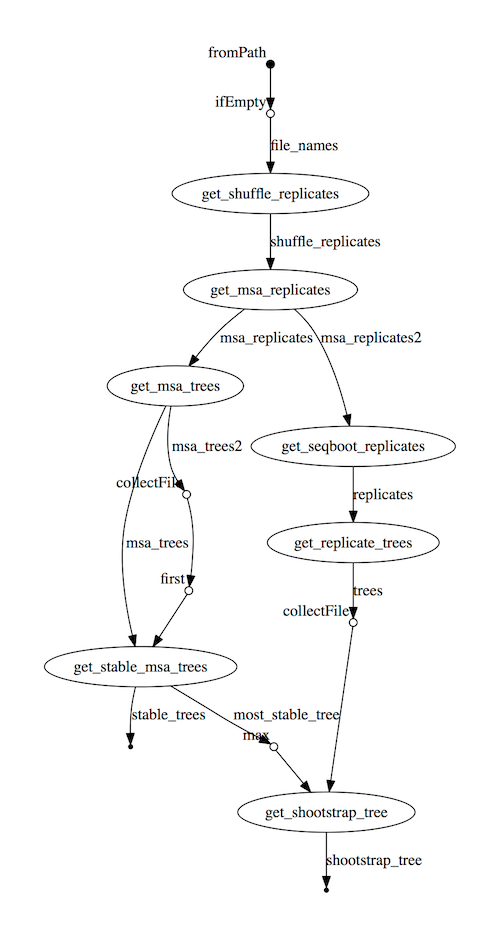
\includegraphics[width=0.45\textwidth,height=0.675\textheight]{fig/dag.png}
        \caption{nf-core/shootstrap Workflow Represented as a Digraph}
        \label{fig:dag}
\end{figure}




%%=========================================
\section{Scientific Workflow Management Systems}
\label{sec:management}

The emergence of scientific workflows as a method for representing and managing these complex computations has lead to the emergence of scientific workflow mangement systems (SWMS, or scientific workflow managers) to manage the execution of scientific workflows and their constituent tasks. Today there are a litany of different SWMS’s, such as Nextflow \cite{nextflow},  Kepler \cite{kepler},  Pegasus \cite{pegasus} and others.

Because the resource requirements of scientific workflows can be immense \cite{ResourceProvisioning}, workflow managers must be able to interface with powerful execution platforms which usually use resource managers such as Kubernetes \cite{kubernetes} or YARN \cite{yarn}. A workflow manager will schedule a workflow’s tasks with the resource manager (this will include assigning the task a fixed amount of resources), handle failures as configured by the user, manage the communication between tasks, and collect and store the results if the workflow’s execution succeeds.

At this point it is important to clarify the distinct responsibilities of a workflow management system, an execution platform and a scientific workflow, with regards to the tasks. The user or creator of the workflow decides which tasks need to be executed and when they need to be executed relative to eachother and the SWMS will schedule tasks with the execution platform according to this design. It is the execution platform which will ultimately decide when a task will actually be executed on physical hardware. In this transaction it is the SWMS which is acting as the middle man. Beyond which tasks to execute, and in which order, the user will also decide what the inputs to a task should be and the workflow manager will ensure that before the task is executed those inputs are available and that they are passed to the task. 

Finally, with regards to resources, the user does not need to specify what the resources assigned to a task should be, the user may do so if they like, however it is not a requirement, and in the event that they do not assign any resources the SWMS will pick an assignment. The assignment of resources to a task is a request by the workflow management system to the execution platform, and, provided the platform can fulfil these requirements, the task should be executed in an environment where it has access to as many resources as it was assigned but not more. Tasks which exceed their resource requirements will often be aborted and this will be communicated to the resource manager which will then have to decided if it should try to run the task again, continue without the task, or abort the execution of the entire workflow- what action to take in this event can also be configured by the user.

%%=========================================
\section{Reinforcement Learning}
\label{sec:rl}

Popularized in the seminal book by Sutton and Barto \cite{sutton_barto}, reinforcement learning can broadly be said to present a framework for a learning system or “agent” to find the optimal policy for achieving a given goal in an uncertain environment by interacting with the problem and the environment. Most importantly it is also able to adjust this policy ``on the go'', meaning it can both learn a new policy if the challenge or the environment changes, and that it can be deployed without any training and it will improve as it gains experience. In this context the agent's goal is always set by a reward function. Using reinforcement learning, the agent learns to maximize this function and thus, hopefully, achieve the desire of its designers. To put it simply, reinforcement learning is a “computational approach to learning from interactions” \cite{sutton_barto}

Central to all reinforcement learning is the idea of exploration versus exploitation. Since the agent initially knows nothing about its environment it must attempt  to learn through exploration. By trying different things and receiving different rewards the agent can construct a policy that always makes the optimal choice. But in order to know what a good or an optimal choice is the learning system must also occasionally make the wrong choice so that it can learn not to make it again. Trying different things is ''exploration'' and using the knowledge gained from this to make the right choice is``exploitation''. An agent cannot simultaneously explore and exploit. This dichotomy is at the core of reinforcement learning. The agent must always make the choice between exploring more to potentially discover an even better policy and eventually yield even better rewards in the future, or using its current policy to increase its immediate rewards.

Beyond the dichotomy mentioned above, the other challenge presented to the designers of a reinforcement learning agent is the question of how to translate the overarching goals into a singular reward. A reinforcement learning agent run ad infinitum should converge to an optimal policy which maximises reward, and thus the onus is on the designer to pick a reward function which, when maximised, will help them to achieve their goals. 

\subsection{Actions, States, Policies and Rewards}
\label{subsec:agent}

For the purposes of this thesis only q-learning and gradient bandits will be discussed. In order to understand these approaches the concepts of states and actions must be introduced. An agent interacts with its environment by performing actions. These actions may have a tangible effect on the agent and the environment and the agent receives feedback about its actions. This feedback is given to the agent in the form of rewards. The agent also maintains an internal representation of itself (either independently or in relation to the environment), this representation is considered the agent’s state. An agent may change states either as a result of its own actions or as a result of changes in the external environment. A simple visual representation of these interactions can be seen in \ref{fig:agent}.

\begin{figure}[htp]
    \centering
        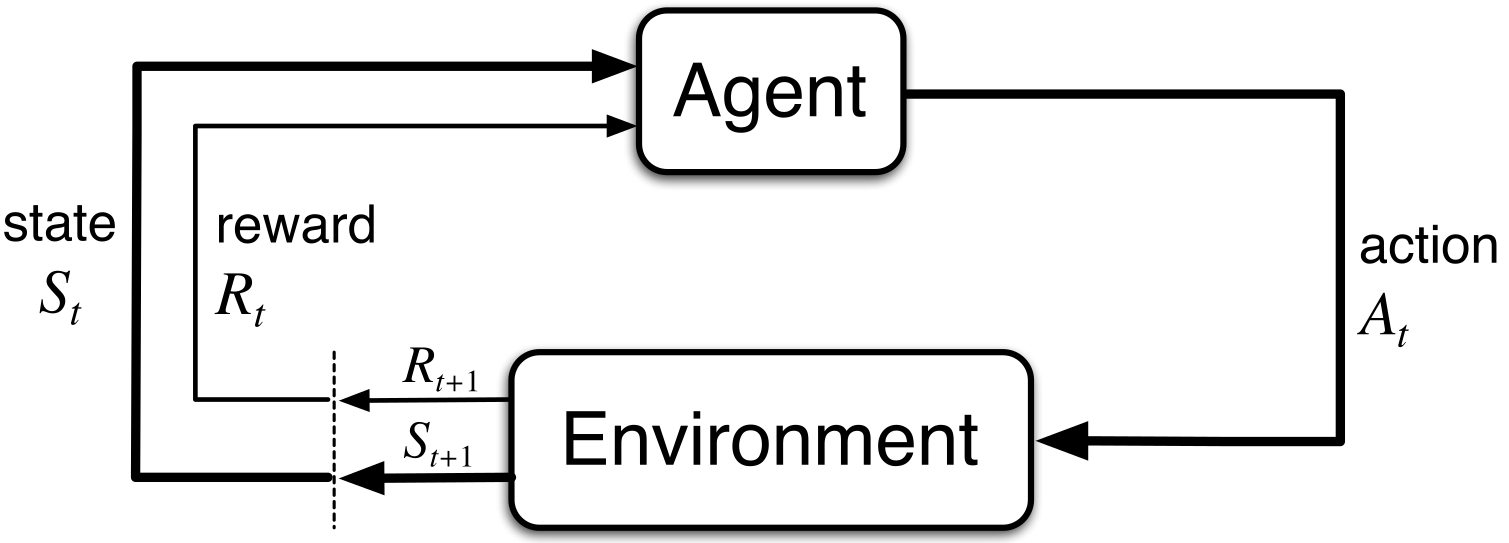
\includegraphics[width=.65\textwidth]{fig/agent.png}
        \caption{Agent Environment Interactions \cite{sutton_barto}}
        \label{fig:agent}
\end{figure}

Policies and the question of how best to evaluate them are crucial to reinforcement learning. Within the context of states, actions and rewards, a policy is simply an instruction for which actions must be taken in which states to maximise the cumulative reward over time. Which action to take may depend on the value of the current state or the value of the state which the action may cause the agent to transition to. In order to achieve its goal an agent needs to develop a policy that maximizes its reward, then as the agent encounters new situations it simply follows the policy it has learned. 

To evaluate a given policy it must be compared to the optimal policy. For any given problem and its reward function there exists at least one policy which maximizes the reward received and is considered optimal. At its core, reinforcement learning aims to enable the agent to continuously refine its current policy so that it approaches the optimal policy. 

\subsection{Gradient Bandits}
\label{subsection_gradient_bandits}

In this thesis two specific types of reinforcement learning are considered. First are gradient bandits. The ``Bandit Problem'' is a sequential learning problem, where each round the bandit has to decide which action to take by pulling one of $N$ levers \cite{ding_efficient}. The analogy used by Sutton and Barto is of a room with several levers, and the question of which lever to pull (the pulling of a certain lever may also be called the action). From the bandit's perspective pulling any of the levers yields a certain reward and it is the bandit's task to find a policy for pulling levers which yields the maximum reward.  Approaches to solving the bandit problem present frameworks for solving problems in which an actor repeatedly returns to a static situation with the same choices. 

Applying this to the case of scientific workflow managers and the sizing of tasks one can consider the levers, or the choice, as the resource configuration. The bandit is asked repeatedly to allocate a certain amount of resources for a task (equivalent to pulling one of the levers) and must find the best policy for maximising the reward (i.e. the best “lever” or resource allocation). 

Gradient bandits solve the bandit problem by using the gradient of the reward function to learn a preference $H_t(a)$ for each of the available actions (or levers). This preference $H_t(a)$ is updated after each round $t$. Using gradient ascent the bandits take small steps in the direction of the ideal preference for each lever to maximize rewards. These steps are taken via stochastic gradient ascent, for which the formula is : 

\begin{equation}\label{gradient_ascent}
H_{t+1}(a) = H_t(a) + \alpha \frac{ \delta E[R_t] }  {\delta H_t(a)}
\end{equation}

Here $E[R_t]$ is the expected reward function and $\alpha$ is the step size.

This formula aims to increment the preference for an action proportional to the increment's effect on performance. The preferences influence the bandit’s probability of choosing a given action. After choosing an action and receiving a reward, the preferences for all of the actions are updated to try and follow the gradient of the reward. 

In practice however the expected reward for each action is not known- if it were known the problem would be trivial and the agent could be configured to always pick the maximizing action. Instead the expected reward function and its gradient must be approximated over time. This leads to the formula for updating the preferences proposed by Sutton and Barto. For a preference $H_{t+1}(A)$ after taking action $A$ at timepoint $t$ (denoted by $A_t$) and receiving reward $R_t$ , where $\hat{R}$ is the average of all the rewards so far and $\pi_t(a_t)$ is the probability of picking action $a_t$, its preferences are updated as follows: 

\begin{align} \label{preference_update}
H_{t+1}(A_t) &= H_t(A_t) + \alpha (R_t - \hat{R}) (1 - \pi_t(A_t)) & \text{and} \\
H_{t+1}(a) &= H_t(a) - \alpha (R_t - \hat{R})\pi_t(a) & \forall a \neq A_t
\end{align}

In this formula $\alpha$ is called the step size and it is a parameter which may be a constant or a function of the time $t$, but it must be greater than 0. It has been proven in \cite{sutton_barto} that this formula eventually approximates formula \ref{gradient_ascent} for gradient ascent. 

After updating its preferences, the gradient bandit then uses these preferences to inform the probability of choosing the next action at time $t+1$. This can be done, for example, using a softmax distribution, and indeed in the rest of this thesis the softmax formula in \ref{softmax} is what is used to update gradient bandits.

\begin{equation}\label{softmax}
\pi_t(a) = \frac {e^{H_t(a)}} {\sum_{i=1}^n e^{H_t(i)}}
\end{equation}

At the start (timepoint $t = 1$) the gradient bandit’s preferences are all the same: $H_1(a_1) = 0 , \forall a$. It then chooses actions based on the probabilities determined by the preferences for each action, updates its preferences with the reward it received according to \ref{preference_update}, and uses \ref{softmax} to update the probabilities, which in turn will determine the next action chosen. Through this method the gradient bandit will begin with a natural inclination to explore, and as it figures out which actions yield the greatest rewards, the probability of picking those actions will increase and the bandit will choose those actions more often, thus naturally striking a balance between exploitation and exploration. 

It should be mentioned, however, that this balance is dependent on the step size $\alpha$. For large values of $\alpha$ the bandit will spend less time exploring and more time exploiting. But despite this, if the nature of the rewards received for a given action begin to change, for example if an action goes from consistently receiving quite large rewards to consistently receiving poor rewards, then the formula in \ref{preference_update} will naturally begin to decrease its preference for that action and the bandit will begin exploration again- regardless of step size. This is one of the strengths of reinforcement learning: it can adapt to changes in the environment or the reward function.

Finally, some terminology- when the preference for an action has become so large that the probability of picking this action approaches 1, then the gradient bandit can be said to have “converged” to this action. 

\subsection{Q-learning}

While the bandits in the previous section do not have a concept of state and must only learn about the actions available to them, stateful agents must maintain an internal state $s \in S$ and choose actions $a \in A$ which will yield new rewards and may cause them to transition to new states. The transition to a new state may also be independent of the action picked. The set of all possible states which the agent may conceivably find itself in and the set of available actions which the agent may potentially take are denoted as $S$ and $A$ respectively. Within this context of states and actions, a policy $\pi(s)$ must pick the agent’s action $a$ based on its current state $s$.

Q-learning was first proposed in \cite{watkins_dayan} and it provides a simple way for an agent to act optimally in controlled Markovian domains \cite{watkins_dayan}. An explanation of Markov domains or policy evaluation is beyond the scope of this thesis. Q-learning will therefore be explained within the context of the simplified agent-environment interface mentioned earlier (subsection \ref{subsec:agent} and figure \ref{fig:agent}). 

Q-learning is an off-policy temporal  difference control algorithm. An in depth explanation of temporal difference is also out of the scope of this thesis but a simplified explanation will come later in this section. Off-policy refers to the fact that q-learning is able to approximate the optimal action-value function independent of the policy being followed. The fundamental formula underpinning q-learning is called one step q-learning:

\begin{equation}\label{eq:q-learning}
Q_{t+1}(s,a) = Q_t(s,a) + \alpha \times (r + \gamma \times max_{\hat{a}}(Q_t(\hat{s},\hat{a})) - Q_t(s,a) )\\
\end{equation}

In this formula the function $Q_t(s,a)$ is a state-action value function. It reflects the value (which is based on both the historic rewards up to timepoint $t$ and the expected future rewards) of taking action $a$ in state $s$. When an agent takes action $a$ it will receive reward $r$ and transition to state $\hat{s}$. After this the agent must update its $Q_t(s,a)$ function to $Q_{t+1}(s,a)$. If the old value function for $s$ and $a$ was $Q_t(s,a)$ then the update to this function is the difference between the old valuation, and the reward plus the discounted expected value of the new state. The expected value of the new state is $Q_t(\hat{s},\hat{a})$, where $\hat{a}$ is the action which maximises $Q_t(\hat{s},a)$ and $\gamma \in [0,1]$ is the discount. This is called the temporal difference:

\begin{equation}\label{eq:TD}
(r + \gamma \times max_{\hat{a}}(Q_t(\hat{s},\hat{a})) - Q_t(s,a)\\
\end{equation}

The temporal difference reflects the difference between the current approximation of the value function ($Q_t(s,a)$) and the optimal value function ($r + \gamma \times Q_t(\hat{s},\hat{a})$). If the current approximation is too optimistic then \ref{eq:TD} will be negative and if $Q_t$ is too pessimistic (too small) then the temporal difference will be positive. $Q_t$ is then adjusted by the temporal difference multiplied with the step size $\alpha$ to yield $Q_{t+1}$. This is what equation \ref{eq:q-learning} does. The only requirement for this iterative process to converge to the optimal value function is that all $(s,a)$ pairs continue to be updated \cite{sutton_barto}.

Using a value function built from equation \ref{eq:q-learning} an agent can approximate an optimal policy by simply using a greedy approach and always picking the action $a$ which maximises $Q(s,a)$, when it is in state $s$ (and then updating its value function according to \ref{eq:q-learning}). Building on this idea, the epsilon greedy q-learning algorithm can be constructed. The pseudocode for this algorithm can be seen below.
\begin{algorithm}[h]
Initialise $Q(s,a) = 0$ , $\forall (s,a)$\\
Initialise start state $s$\\
\While{\textbf{True}}{
        \eIf{$random < \epsilon$}{choose action $a$ randomly}{choose action $a = max_a (Q(s,a))$}
        Take action $a$, receive reward $r$, transition to state $\hat{s}$\\
        Update $Q$: $Q_{new}(s,a) = Q(s,a) + \alpha \times (r + \gamma \times max_{\hat{a}}(Q(\hat{s},\hat{a})) - Q(s,a) )$\\
}
\caption{Epsilon Greedy Q-learning Pseudocode}
\label{alg:q-learning}
\end{algorithm}

This algorithm introduces random exploration with a probability $\epsilon$ and follows the q-learning algorithm the rest of the time. With sufficient exploration and an epsilon that eventually decreases to zero this algorithm should approximate an optimal value function and can greedily select those actions which maximise the $Q$ function it is learning. This is the algorithm which will be used by all q-learning agents implemented in this thesis. 

A final note: since the requirement for convergence to the optimal value function is that all pairs are visited, during early runs whenever the q-learning agent encounters a situation with an action it has never chosen before, it must choose this action. Only if all the available actions have been tried at least once can it use the greedy approach of selecting the maximising action.

Similar to subsection \ref{subsection_gradient_bandits} the q-learning agent also has a step size parameter $\alpha$, and the agent also has to balance exploration against exploitation. However for the q-learning agent its exploration can be directly influenced by the $\epsilon$ parameter, whereas the gradient bandit’s exploration is implicitly tied to its preferences.

